\section{Date: 2026-11-23}
\noindent \textbf{Series ID: PECIUB0T4DC11000A647NCEN} 

\noindent This series is titled 90\% Confidence Interval Upper Bound of Estimate of People Under Age 5 in Poverty for District of Columbia and has a frequency of Annual. The units are Persons and the seasonal adjustment is Not Seasonally Adjusted.The observation start date is 1989-01-01 and the observation end date is 2024-01-01.The popularity of this series is 1. \\ 

\noindent \textbf{Series ID: AUTHNOT24USA} 

\noindent This series is titled New Privately-Owned Housing Units Authorized but Not Started: Units in Buildings with 2-4 Units and has a frequency of Monthly. The units are Thousands of Units and the seasonal adjustment is Seasonally Adjusted.The observation start date is 1999-01-01 and the observation end date is 2026-10-01.The popularity of this series is 2. \\ 

\subsection{Raw Regression}
\noindent Regresses the two series against each other directly. A significant result here can come just as easily from both series sharing a long-run trend as from any real relationship.

\begin{center}
\begin{tabular}{lclc}
\toprule
\textbf{Dep. Variable:}                        & value\_fred\_AUTHNOT24USA & \textbf{  R-squared:         } &     0.001   \\
\textbf{Model:}                                &            OLS            & \textbf{  Adj. R-squared:    } &    -0.041   \\
\textbf{Method:}                               &       Least Squares       & \textbf{  F-statistic:       } &   0.02204   \\
\textbf{Date:}                                 &      Mon, 23 Nov 2026     & \textbf{  Prob (F-statistic):} &    0.883    \\
\textbf{Time:}                                 &          22:59:37         & \textbf{  Log-Likelihood:    } &   -56.977   \\
\textbf{No. Observations:}                     &               26          & \textbf{  AIC:               } &     118.0   \\
\textbf{Df Residuals:}                         &               24          & \textbf{  BIC:               } &     120.5   \\
\textbf{Df Model:}                             &                1          & \textbf{                     } &             \\
\textbf{Covariance Type:}                      &         nonrobust         & \textbf{                     } &             \\
\bottomrule
\end{tabular}
\begin{tabular}{lcccccc}
                                               & \textbf{coef} & \textbf{std err} & \textbf{t} & \textbf{P$> |$t$|$} & \textbf{[0.025} & \textbf{0.975]}  \\
\midrule
\textbf{const}                                 &       4.5673  &        3.847     &     1.187  &         0.247        &       -3.372    &       12.507     \\
\textbf{value\_fred\_PECIUB0T4DC11000A647NCEN} &   -5.044e-05  &        0.000     &    -0.148  &         0.883        &       -0.001    &        0.001     \\
\bottomrule
\end{tabular}
\begin{tabular}{lclc}
\textbf{Omnibus:}       & 11.069 & \textbf{  Durbin-Watson:     } &    0.352  \\
\textbf{Prob(Omnibus):} &  0.004 & \textbf{  Jarque-Bera (JB):  } &    9.552  \\
\textbf{Skew:}          &  1.380 & \textbf{  Prob(JB):          } &  0.00843  \\
\textbf{Kurtosis:}      &  4.094 & \textbf{  Cond. No.          } & 9.85e+04  \\
\bottomrule
\end{tabular}
%\caption{OLS Regression Results}
\end{center}

Notes: \newline
 [1] Standard Errors assume that the covariance matrix of the errors is correctly specified. \newline
 [2] The condition number is large, 9.85e+04. This might indicate that there are \newline
 strong multicollinearity or other numerical problems.

\begin{figure}
\centering
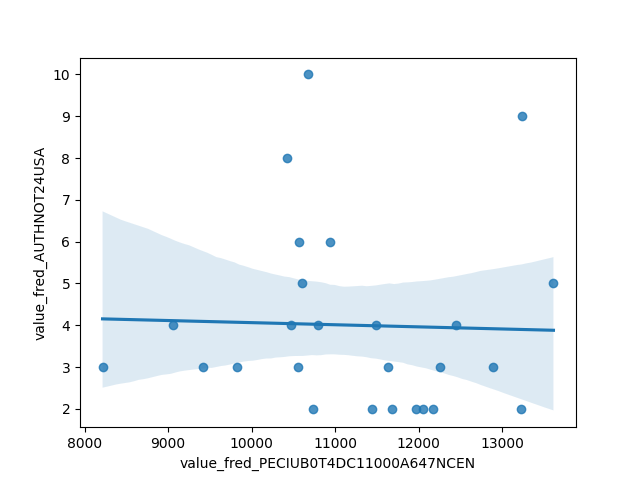
\includegraphics[scale = 0.9]{plots/plot_2026-11-23.png}
\caption{Raw Regression Plot for 2026-11-23}
\end{figure}
\newpage
\subsection{Detrended Regression}
\noindent Regresses the residuals of each series after removing its own linear time trend, so a shared trend can no longer drive the result on its own. A relationship that stays significant here is better evidence of a genuine link between the two series.

\begin{center}
\begin{tabular}{lclc}
\toprule
\textbf{Dep. Variable:}                                   & value\_fred\_AUTHNOT24USA\_detrended & \textbf{  R-squared:         } &     0.020   \\
\textbf{Model:}                                           &                 OLS                  & \textbf{  Adj. R-squared:    } &    -0.021   \\
\textbf{Method:}                                          &            Least Squares             & \textbf{  F-statistic:       } &    0.4890   \\
\textbf{Date:}                                            &           Mon, 23 Nov 2026           & \textbf{  Prob (F-statistic):} &    0.491    \\
\textbf{Time:}                                            &               22:59:37               & \textbf{  Log-Likelihood:    } &   -55.392   \\
\textbf{No. Observations:}                                &                    26                & \textbf{  AIC:               } &     114.8   \\
\textbf{Df Residuals:}                                    &                    24                & \textbf{  BIC:               } &     117.3   \\
\textbf{Df Model:}                                        &                     1                & \textbf{                     } &             \\
\textbf{Covariance Type:}                                 &              nonrobust               & \textbf{                     } &             \\
\bottomrule
\end{tabular}
\begin{tabular}{lcccccc}
                                                          & \textbf{coef} & \textbf{std err} & \textbf{t} & \textbf{P$> |$t$|$} & \textbf{[0.025} & \textbf{0.975]}  \\
\midrule
\textbf{const}                                            &   -1.726e-13  &        0.416     & -4.15e-13  &         1.000        &       -0.858    &        0.858     \\
\textbf{value\_fred\_PECIUB0T4DC11000A647NCEN\_detrended} &      -0.0002  &        0.000     &    -0.699  &         0.491        &       -0.001    &        0.000     \\
\bottomrule
\end{tabular}
\begin{tabular}{lclc}
\textbf{Omnibus:}       &  7.541 & \textbf{  Durbin-Watson:     } &    0.419  \\
\textbf{Prob(Omnibus):} &  0.023 & \textbf{  Jarque-Bera (JB):  } &    5.715  \\
\textbf{Skew:}          &  1.092 & \textbf{  Prob(JB):          } &   0.0574  \\
\textbf{Kurtosis:}      &  3.711 & \textbf{  Cond. No.          } & 1.24e+03  \\
\bottomrule
\end{tabular}
%\caption{OLS Regression Results}
\end{center}

Notes: \newline
 [1] Standard Errors assume that the covariance matrix of the errors is correctly specified. \newline
 [2] The condition number is large, 1.24e+03. This might indicate that there are \newline
 strong multicollinearity or other numerical problems.

\begin{figure}
\centering
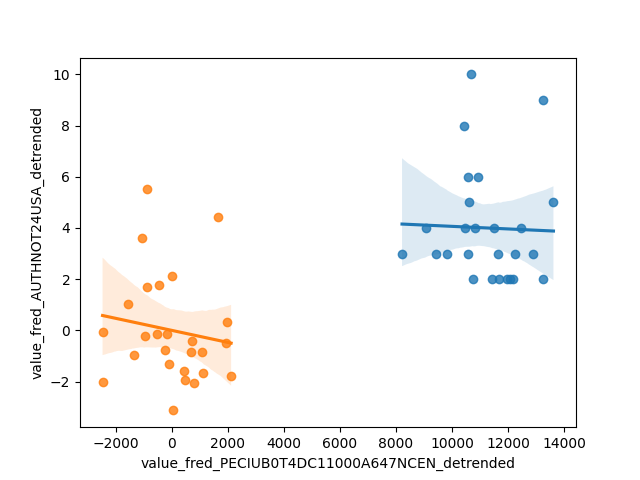
\includegraphics[scale = 0.9]{plots/plot_2026-11-23_detrended.png}
\caption{Detrended Regression Plot for 2026-11-23}
\end{figure}
\newpage
